\subsubsection{Attenuation length and effective speed of light}
\label{sect:att_speed}

% plots needed ADC LanGaus fit, smoothed ADC with maximum position, att length vs set number

The scintillator material for the TOF system must have short decay times, long attenuation
length, and good spectral match to the PMTs. Initial measurements show that attenuation
length values vary even among scintillation bars of the same material and from the
same mold, so in order to verify that each counter meets required specifications, the attenuation
length measurement is incorporated into the unit testing of each counter constructed
for Panel 1B. The method uses the same data collected in the six-bar time resolution
measurements described in Sec.~\ref{sect:refin}.	

Firstly the whole bar length was divided into slices by using time-walk corrected TDC difference between left and right PMTs shown on Fig.~\ref{fig:tdc_diff}. Red lines on Fig.~\ref{fig:tdc_diff} correspond to the x-positions of half maxima for left and right slopes of the distribution. The distance between these lines is proportional to the bar length, so after the TDC difference was divided into slices the bar length is also automatically sliced.


\begin{figure}[]
\centering
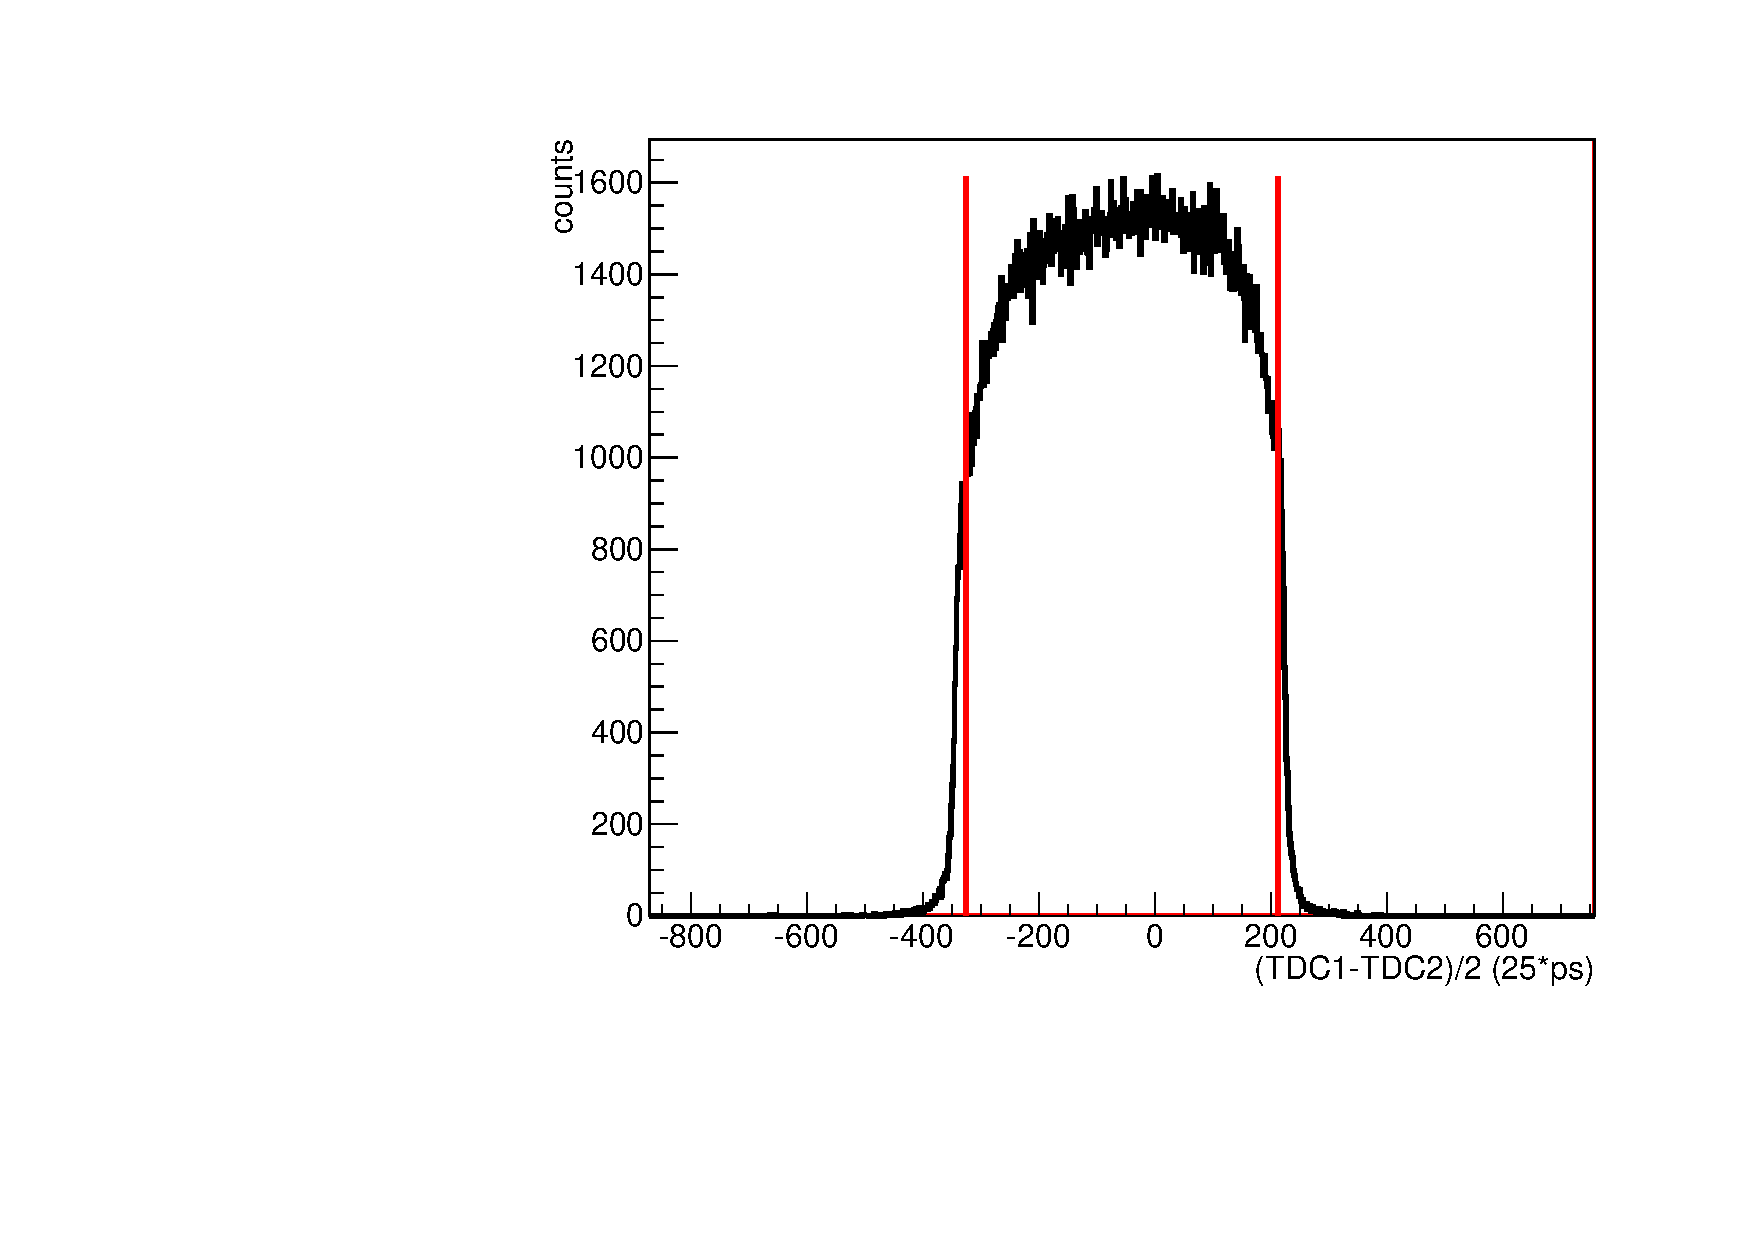
\includegraphics[width=0.6\textwidth]{gleb/fig_gleb_att_length/tdc_diff.pdf}
\caption{Half of the time-walk corrected TDC difference for the bar 200 cm long from the set 30. Vertical red lines correspond to the $x$-positions of half maxima for left and right slopes of the distribution.\label{fig:tdc_diff}}
\end{figure}


For events inside each slice ADC distributions for each PMT were plotted as shown on Fig.~\ref{fig:adc_maximum}. The maximum of each distribution can be determined by two methods. In the first method the position of the maximum can be found either  by fitting
with Landau or Gauss-convoluted Landau functions as it shown on the left side of Fig.~\ref{fig:adc_maximum}. Both functions give relatively the same positions of the maximum, but Gauss-convoluted Landau fit describes data better. In the second method the center of the  maximum bin of the histogram smoothed by running mean procedure is treated as the maximum of the ADC distribution  as shown on the right side of the Fig.~\ref{fig:adc_maximum}. Dashed vertical lines on both plots on Fig.~\ref{fig:adc_maximum} represent peak positions, which are relatively the same for both methods. But since the second method consumes less CPU time it was chosen as preferable to analyze the rest of the data.  

Then obtained maxima positions were plotted versus position along the scintillator length Fig.~\ref{fig:attlength}. Attenuation length was determined by fitting this distribution with convolution of two exponents~(\ref{eq:att}).

\begin{equation}
N = N_{0}^{T}e^{-x/{\lambda_{T}}} +N_{0}^{B}e^{-x/{\lambda_{B}}}, \label{eq:att}
\end{equation} 
where $N_0 = N_0^{T} + N_0^{B}$ is the initial number of photons caused by the cosmic ray passing through the scintillator at the impact position $x$ and $N$ is the number of photons arriving
at the PMT.
Since attenuation length of scintillator can be divided into two parts two exponential functions were used for the fit. One part is called 
the technical attenuation length (TAL), which is defined as the length reducing the amount of
light by a factor $e$ and depends on the geometry of the scintillator and the reflective 
properties of its surface. The other part is called bulk attenuation length (BAL), which reduces the initial light intensity by a factor $e$ according to the Buger-Lambert Law and depends on the transparency and the scintillation material. 


\begin{figure}[]
\centering
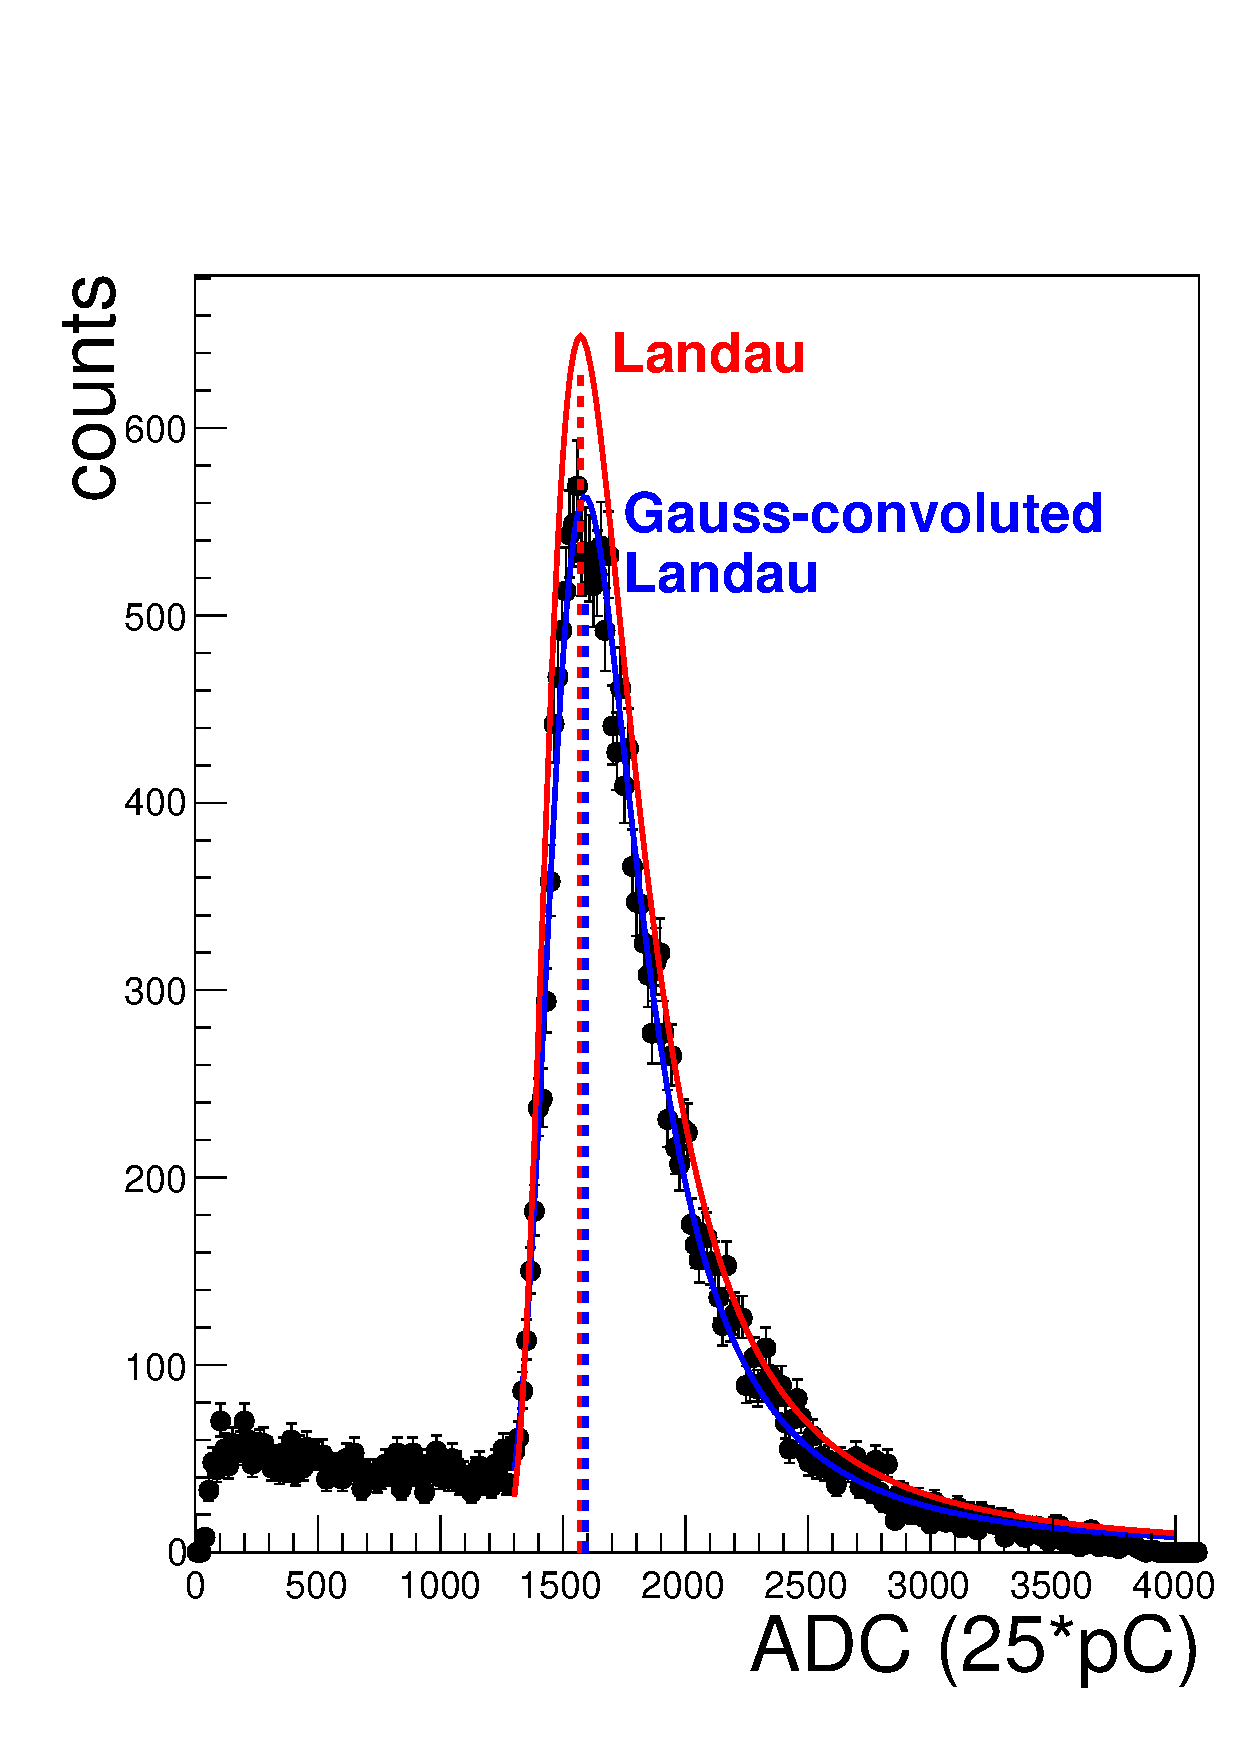
\includegraphics[width=0.4\textwidth]{gleb/fig_gleb_att_length/att_langau.pdf}
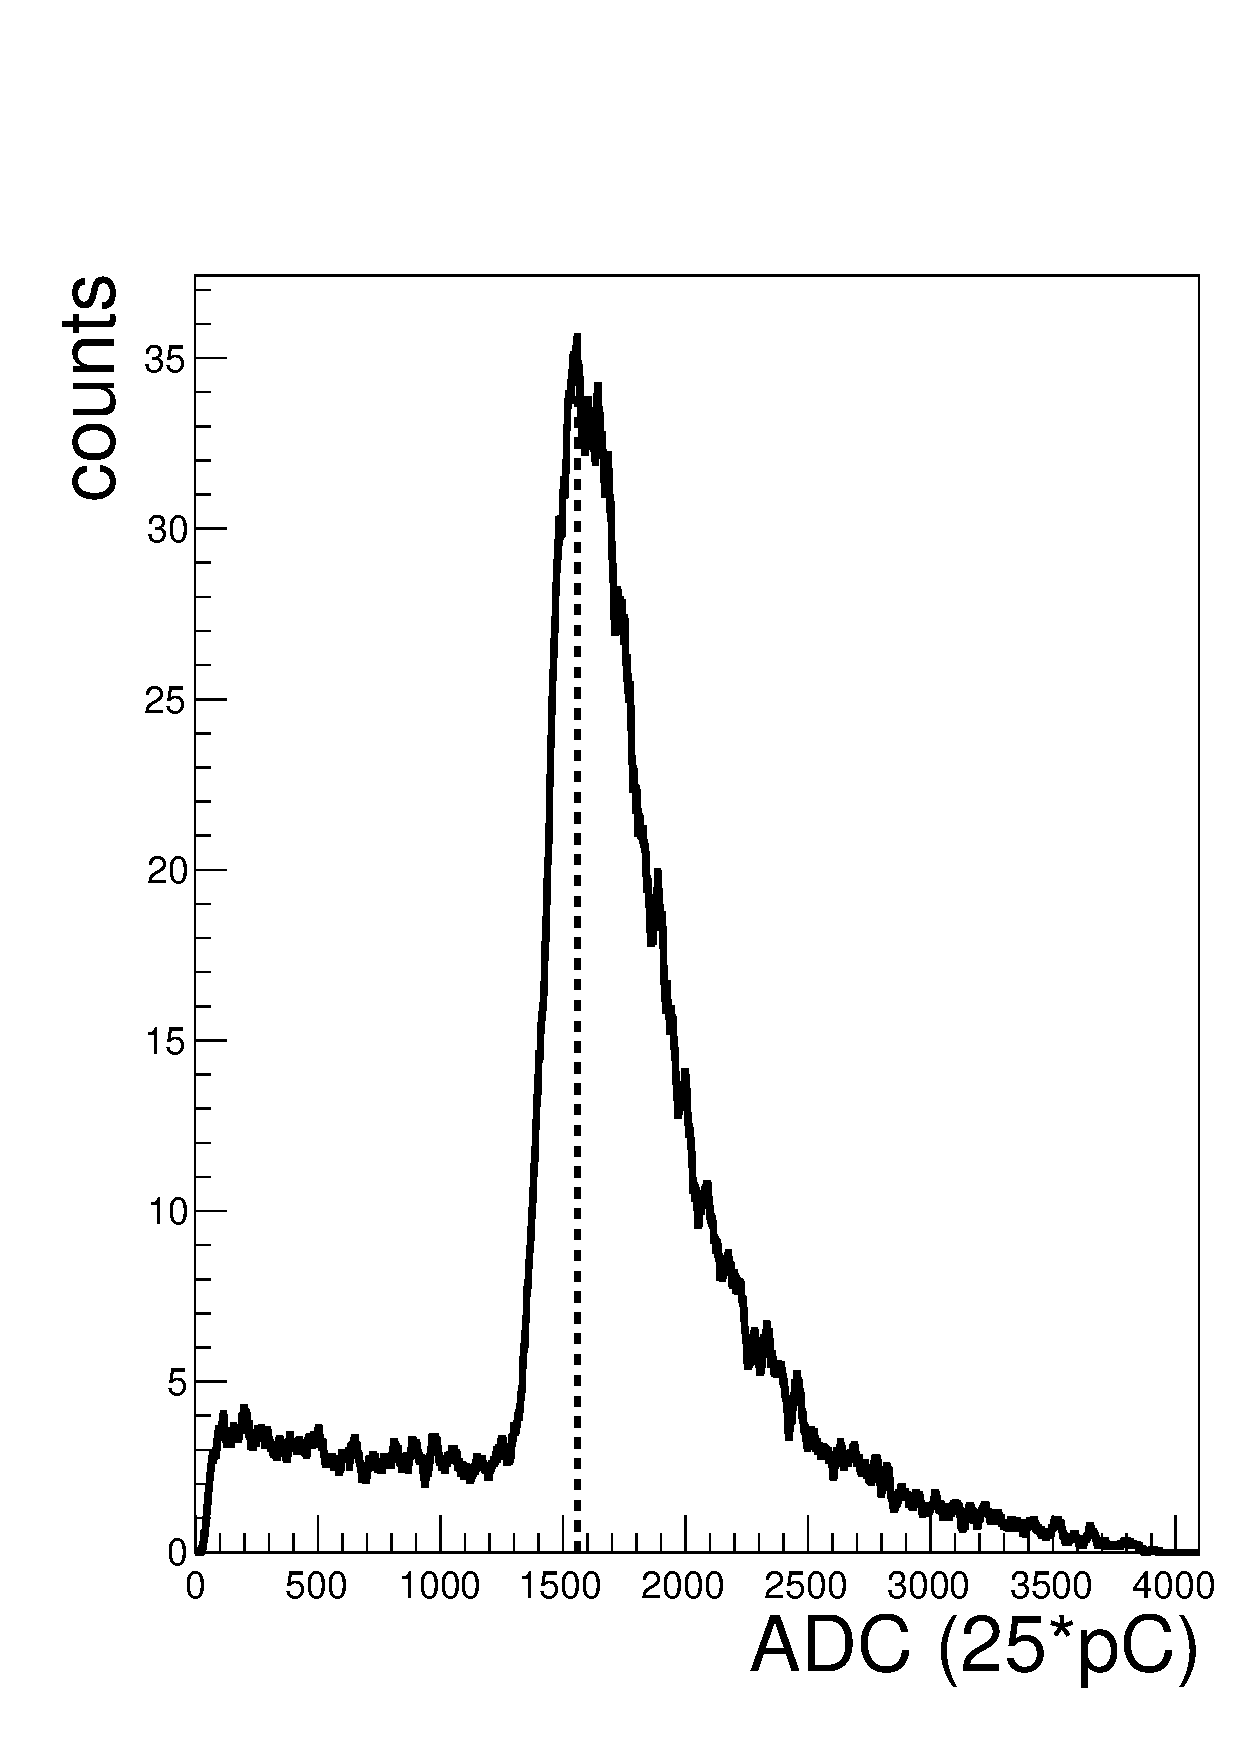
\includegraphics[width=0.4\textwidth]{gleb/fig_gleb_att_length/maximum.pdf}
\caption{ADC distribution for one of the TDC difference slice from the Fig.~\ref{fig:tdc_diff} for one of the PMTs. Left side: Landau fit in comparison with Gauss-convoluted Landau fit. Since 12 bits ADCs was used the histogram had 4096 bins, for illustrative purposes each 16 bins were averaged into one. Dashed vertical lines correspond to the maximum of the distribution given bu the fits. Right side: The same ADC distribution smoothed with by running mean procedure with averaging parameter 30. Dashed vertical line represents the center of the maximum bin.  \label{fig:adc_maximum}}
\end{figure}

In addition to the exponential fit attenuation length was also determined by the two points method, where technical attenuation length is treated as negligible (\ref{eq:att_2_points}). For that purpose $x$ and $y$ coordinates of penultimate points from each side of distribution like Fig.~\ref{fig:attlength} were inserted into equation \ref{eq:att_2_points} instead of $x$ and $N$ correspondingly. After that obtained system of two equations was solved for $\lambda_{2 poins}$.


\begin{equation}
N = N_{0}e^{-x/{\lambda_{2 poins}}}, \label{eq:att_2_points}
\end{equation}

Results for attenuation length obtained from left and right PMT for each bar are almost the same, so finally the averaged value was taken.
On Fig.~\ref{fig:att_vs_barnum} bulk attenuation length is plotted as function of the set number. Various symbols correspond to different scintillators in the set. The gap at set number 32 corresponds to the fact that according to design requirements for short counters, less then 200 cm in length, fast material with short attenuation length is needed, while for long counters scintillators with large attenuation length is the better choice.

\begin{figure}[]
\centering
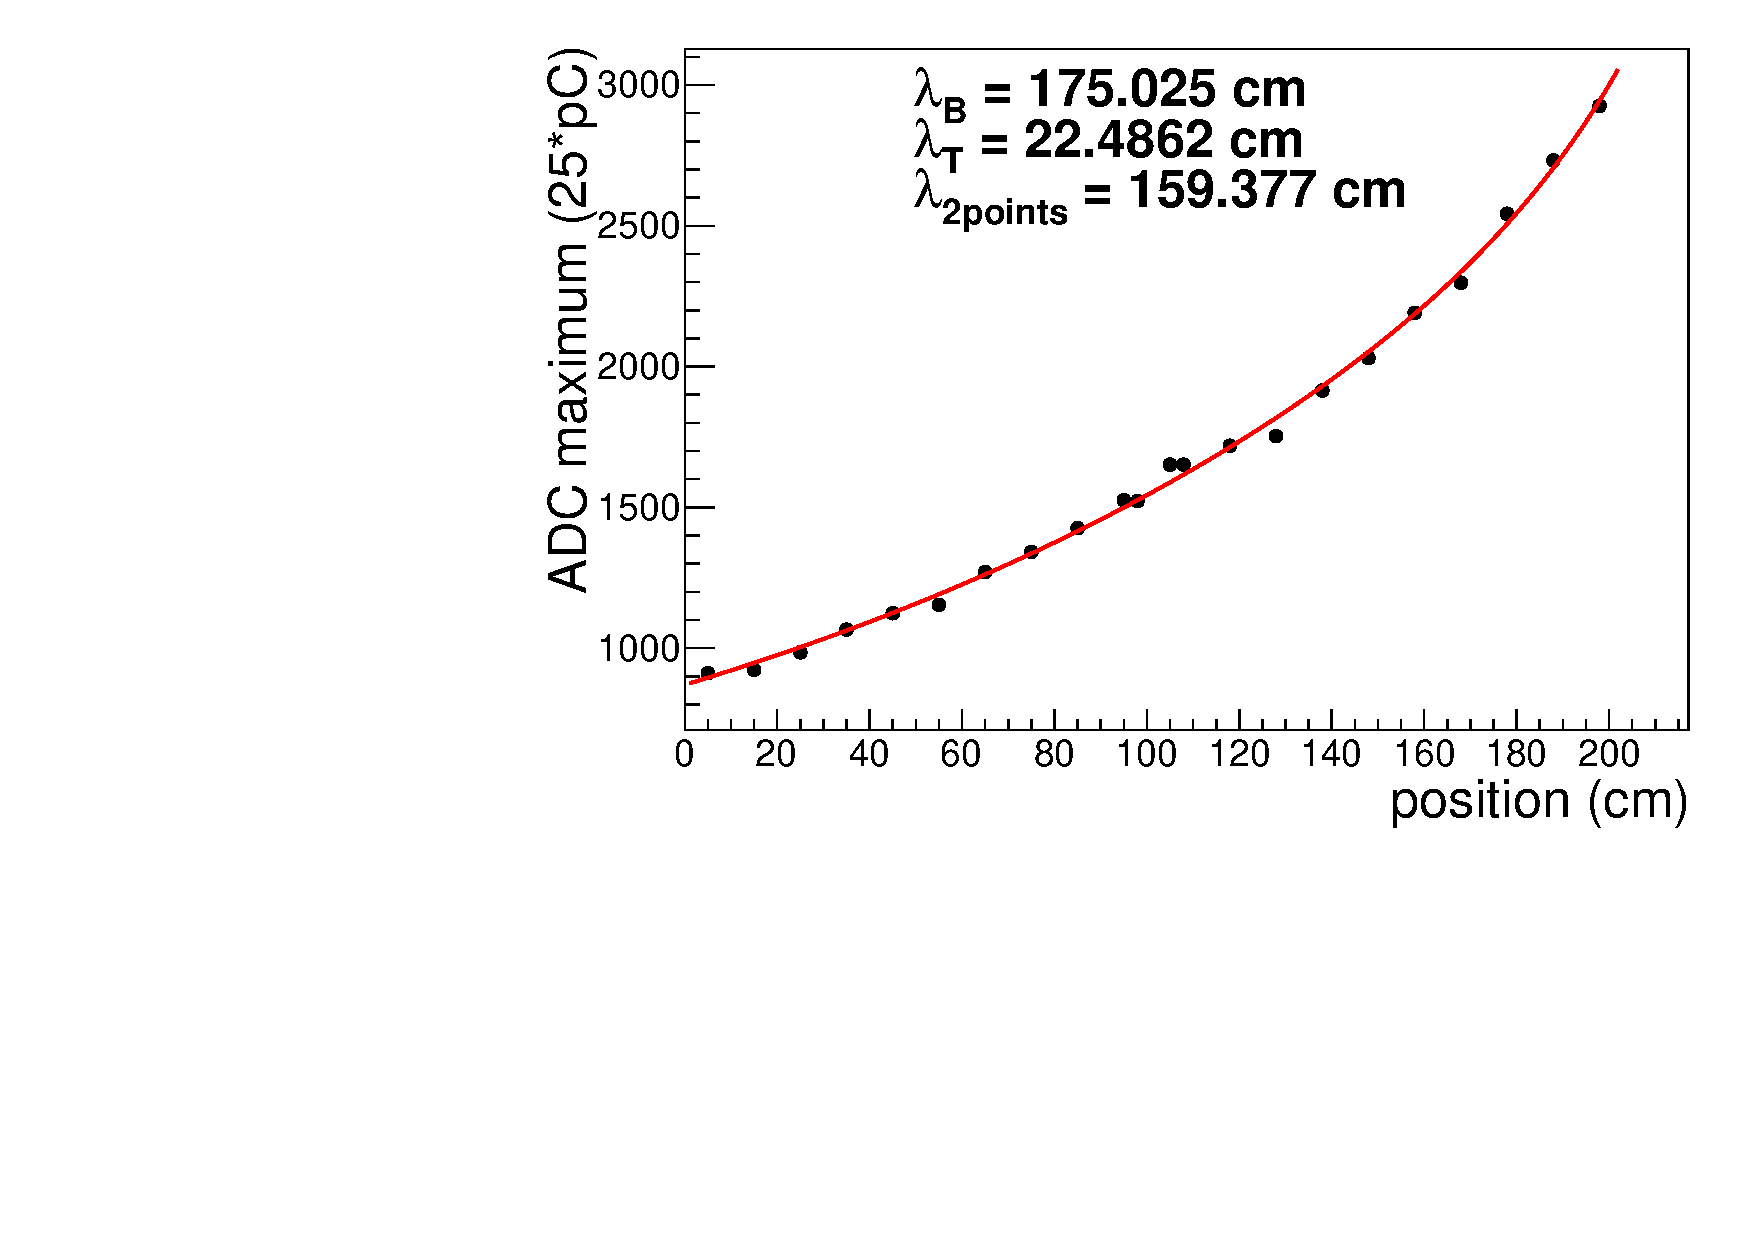
\includegraphics[width=0.6\textwidth]{gleb/fig_gleb_att_length/att_length.pdf}
\caption{Maxima positions of the ADC distributions for one of the PMTs as function of position along the scintillator bar. Red curve represents fit by two exponential function from Eq.~\ref{eq:att}. $\lambda_{B}$ and $\lambda_{T}$ are bulk and technical attenuation lenghtes correspondingly, which were determined from the fit. $\lambda_{2point}$ is bulk attenuation length determined from two penultimate points. \label{fig:attlength}}
\end{figure}


To determine effective speed of light for each scintillator the ratio of bar length, which is known, over the light passing time, which is extracted from TDC values is taken.  Light passing time is determined by the distance between red lines on the Fig.~\ref{fig:tdc_diff}. Effective speed of light for six scintillators from one set is shown on Fig.~\ref{fig:c_eff}. It could be noticed that effective speed of light appears to be slightly higher for bars closest to the center in the six-bar set. This effect can be explained in the following way. Only those tracks that hit all six bars are taken into account, but the behaviour of non-vertical tracks differs from the vertical. Vertical track hits all bars in the set at the same position, but non-vertical track, which hits edges of the top and bottom bars, hits other bars farther form the edges. So, the closer bar to the center of the set the less tracks hit the edges of the bar and the more narrow TDC distribution appears to be.


\begin{figure}[]
\centering
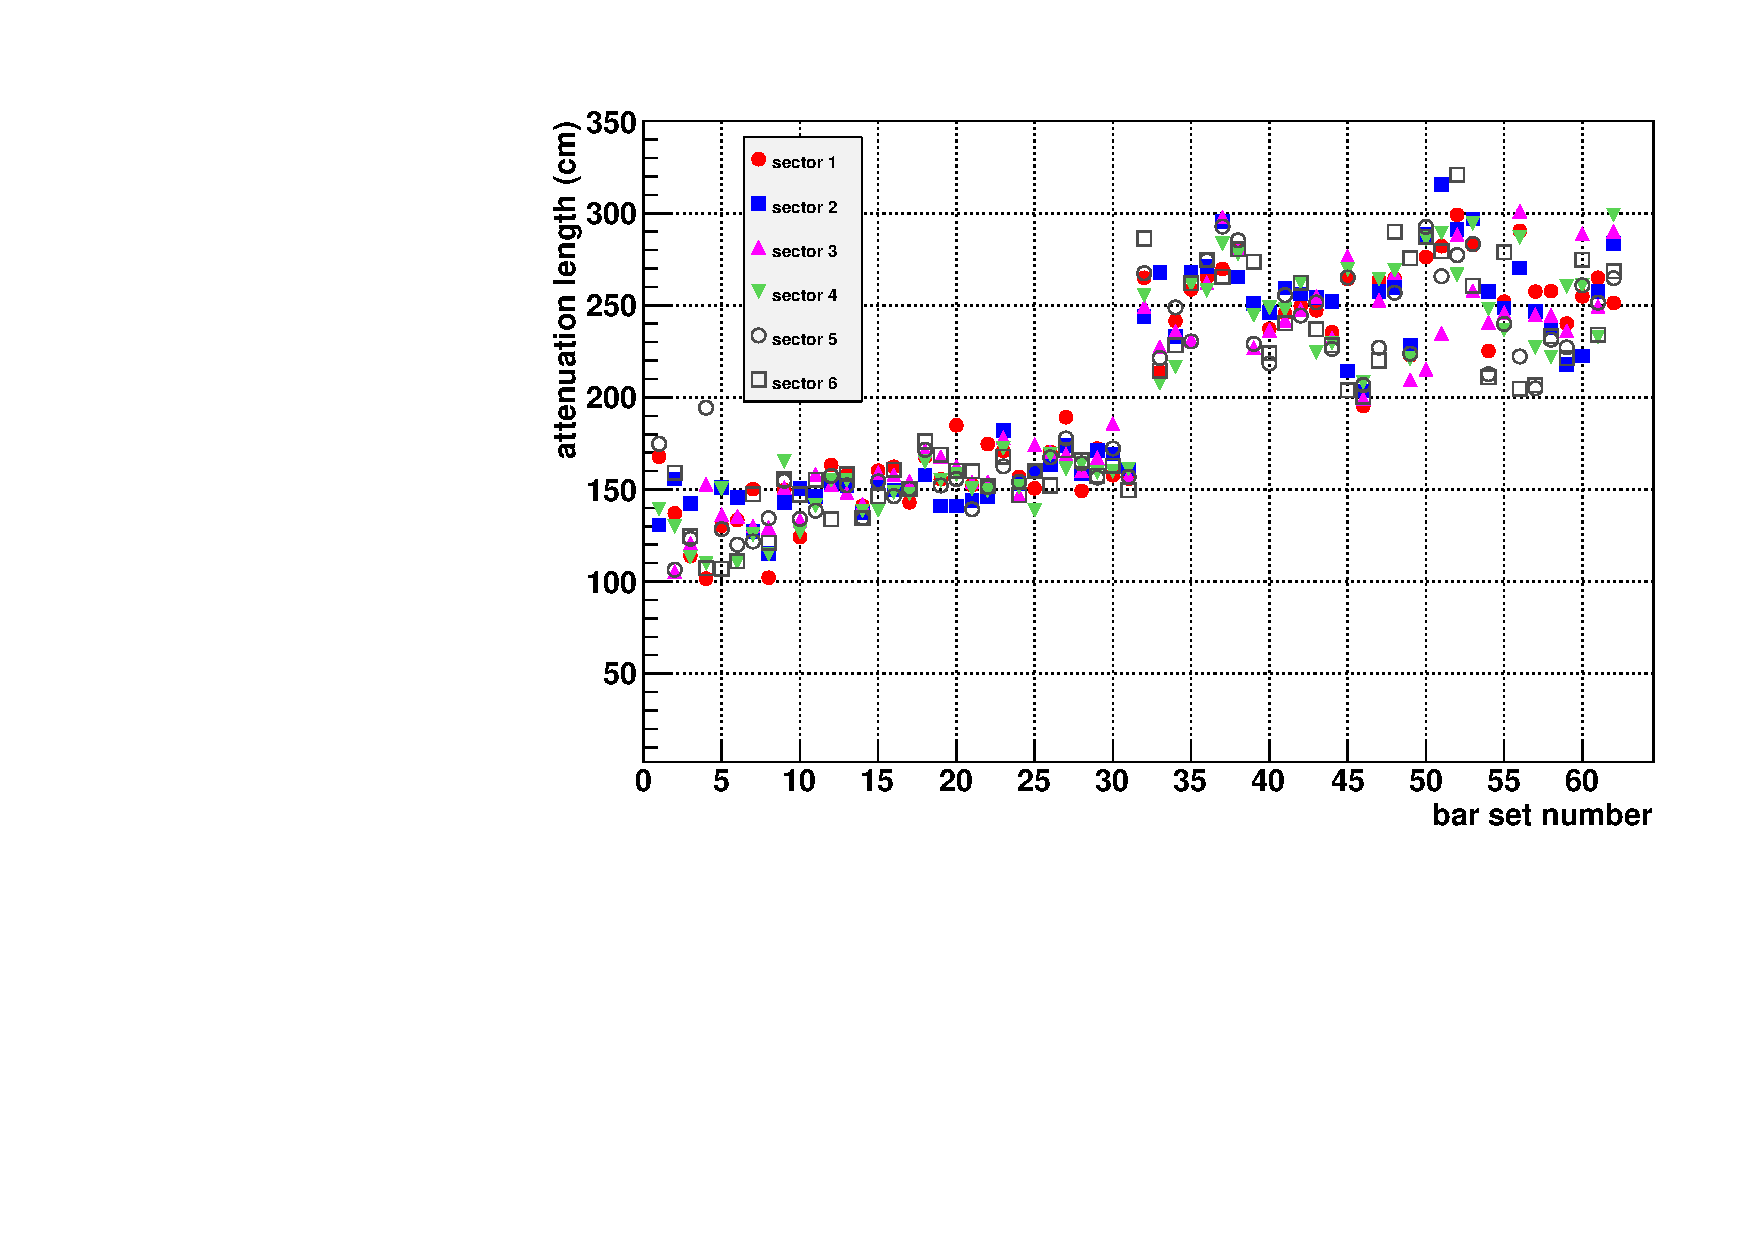
\includegraphics[width=0.8\textwidth]{gleb/fig_gleb_att_length/att_vs_barnum.pdf}
\caption{Averaged bulk attenuation length versus versus set number. Various simbols correspond to the different scintillators in the set or in other words to CLAS12 sectors. \label{fig:att_vs_barnum}}
\end{figure}






\begin{figure}[]
\centering
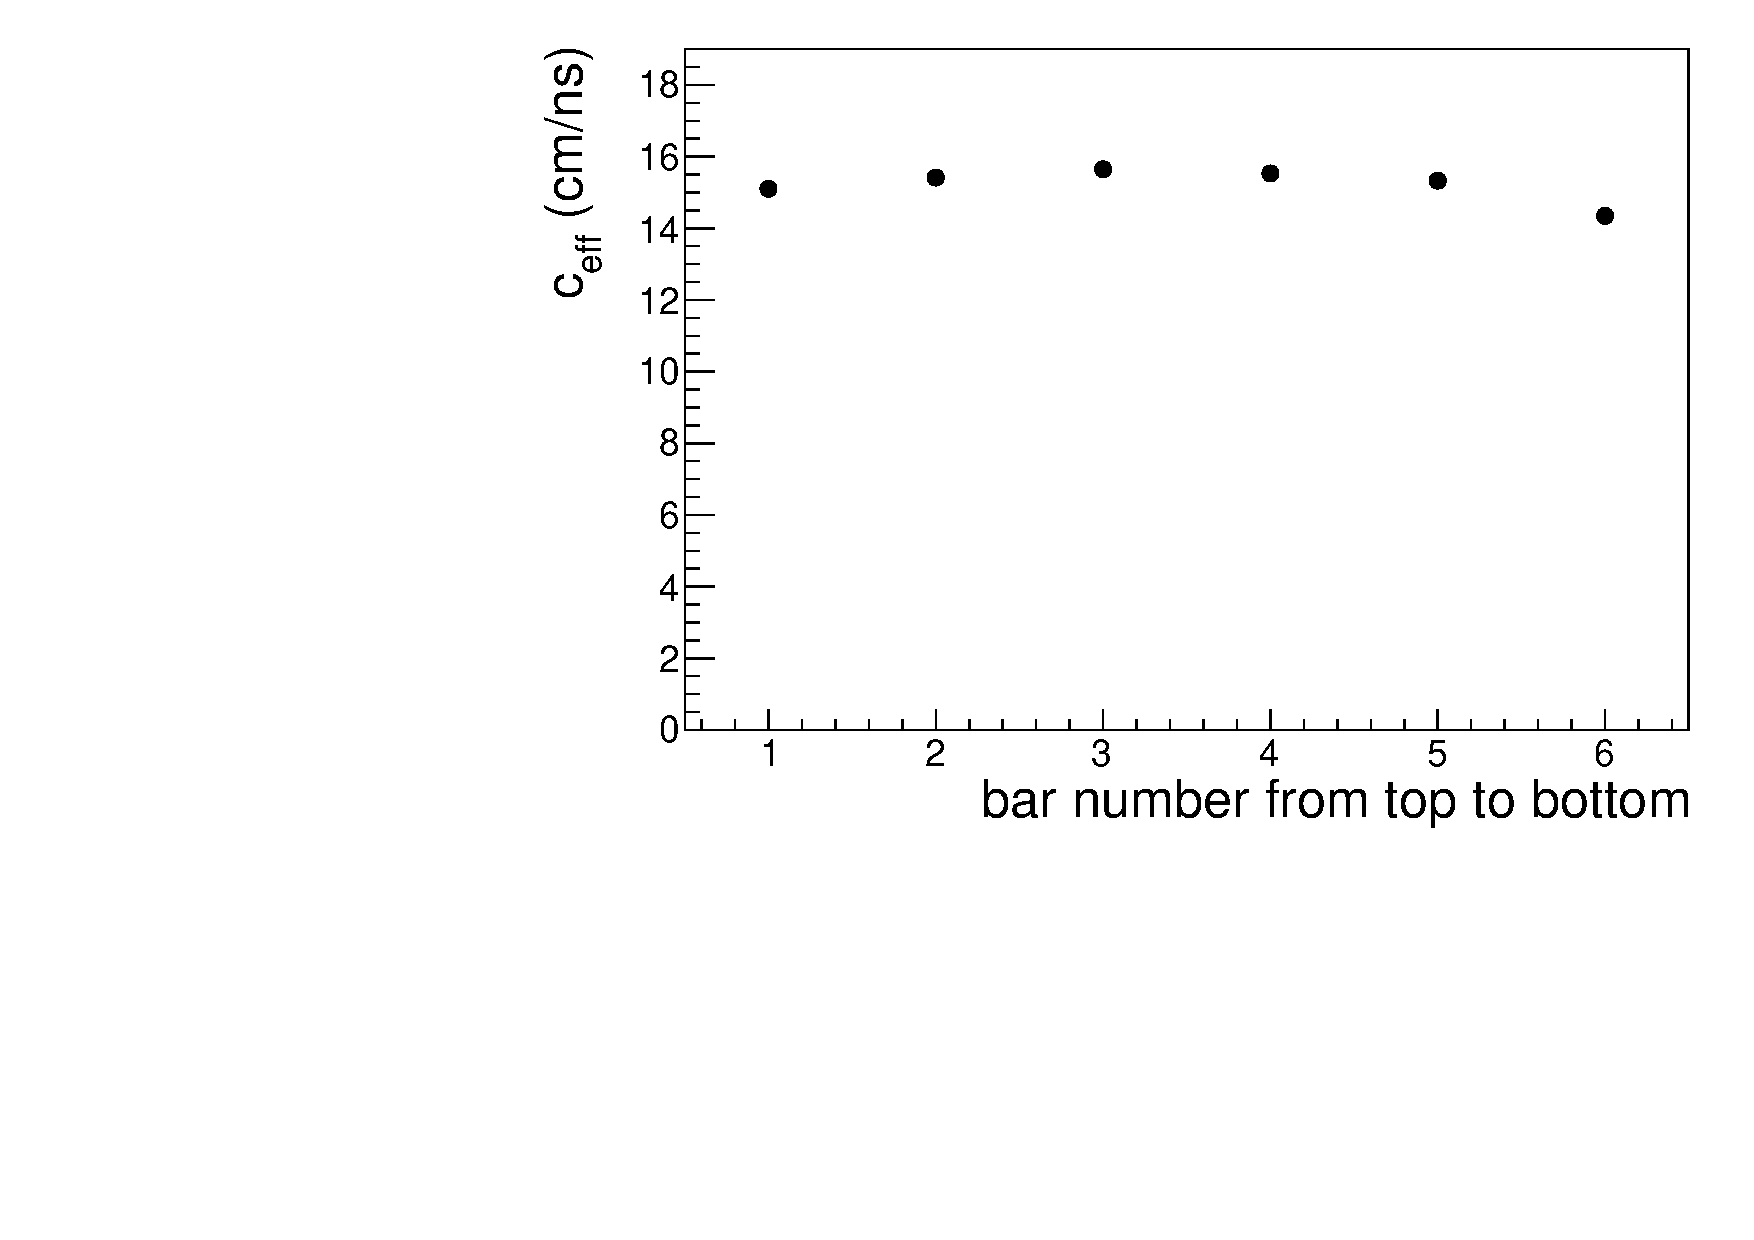
\includegraphics[width=0.6\textwidth]{gleb/fig_gleb_att_length/c_eff.pdf}
\caption{Effective speed of light as function of bar number in the set. Example is given for set number 30. \label{fig:c_eff}}
\end{figure}
